\chapter{Checkpoint-on-Failure}\label{chap:cof}

As a first attempt to meet the goals set out in Chapter~\ref{chap:goals}, we
evaluated the feasibility of implementing fault tolerance in the context of the
current \mpi Standard (version 3.0~\cite{MPI30}), using only the mechanisms 
available as it is currently written. This chapter details that effort and demonstrates 
an application that can function under such constraints.

\section{Existing Error Handling in \mpi}\label{sect:cof:existing}

The existing MPI Standard provides minimal support for fault tolerance. Section
2.8 states in the first paragraph: 

\begin{quote}
MPI does not provide mechanisms for
dealing with failures in the communication system. [\ldots] Whenever possible,
such failures will be reflected as errors in the relevant communication call.
Similarly, MPI itself provides no mechanisms for handling processor failures.
\end{quote}

Failures, be they due to a broken link or a dead process, are considered
resource errors. Later, in the same section: 

\begin{quote}
This document does not
specify the state of a computation after an erroneous MPI call has occurred. The
desired behavior is that a relevant error code be returned, and the effect of
the error be localized to the greatest possible extent.
\end{quote}

So, in the existing
standard, process failures are treated as errors, and therefore the behavior of
the MPI library is undefined. However, the standard does provide guidance for
implementations to be considered ``high quality''. The second excerpt hints at
such behavior by suggesting that the library attempt to localize the impact of
the error and inform the application of the failure. Unfortunately, most of the
implementations of the MPI Standard have implemented process failures as
unrecoverable errors, and the processes of the application are most often killed
by the runtime system when a failure is detected on any of them, leaving no opportunity
for the user to mitigate the impact of failures.

In addition to this limited definition of the behavior of the library after a
process failure, MPI also defines a construct called an
\mpifunc{MPI\_ERRHANDLER}. These are designed to be triggered when a high
quality implementation of MPI detects a failure of some kind. The
\mpifunc{MPI\_ERRHANDLER} is attached to an \mpi Communicator object
and includes a callback function which is executed by the library. MPI provides
two built-in error handlers, \mpifunc{MPI\_ERRORS\_ARE\_FATAL} and
\mpifunc{MPI\_ERRORS\_RETURN}. \mpifunc{MPI\_ERRORS\_ARE\_FATAL} is the default
error handler, and when MPI detects a failure, it automatically aborts the 
entire MPI application without the possibility of recovery or cleanup.
\mpifunc{MPI\_ERRORS\_RETURN} provides more functionality by attempting to
return control to the application after a failure. MPI is no longer usable for
communication, but the application can perform actions to clean up the system
before exiting. Custom error handlers provide the most flexibility. Their 
callback function can perform last second operations as the \mpi library becomes 
unusable.

\section{The Checkpoint-on-Failure Protocol}
\label{sect:cof:protocol}

\begin{table}
	\centering
	\captionof{table}{The Checkpoint-on-Failure Protocol}
	\label{tab:cof:cof}
	\begin{tabular}{|| l | c ||}
		\hline
		& \multirow{9}{*}{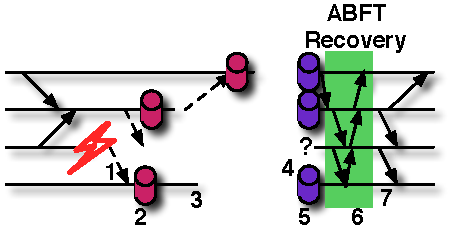
\includegraphics[width=.45\linewidth]{figures/idea.pdf}} \\
		1. MPI returns an error on surviving processes &  \\
		2. Surviving processes checkpoint & \\
		3. Surviving processes exit & \\
		4. A new MPI application is started & \\
		5. Processes load from checkpoint (if any) & \\
		6. Processes enter \abft dataset recovery & \\
		7. Application resumes & \\
		& \\
		\hline
	\end{tabular}
\end{table}

Based on the capabilities of the current version of the MPI Standard, we
designed a new approach for supporting \abft applications, called
Checkpoint-on-Failure (\cof). Table~\ref{tab:cof:cof} presents the steps
involved in the \cof method. In the figure, horizontal lines represent the
execution of processes in two consecutive MPI applications. When a failure
eliminates a process, other processes in the application are notified and regain control from
ongoing MPI calls (1). Surviving processes should assume the MPI library is
dysfunctional and not continue to use MPI operations (in particular, they do
not yet undergo \abft recovery). Instead, they checkpoint their current state
independently (2) and abort (3). If any processes were not initially alerted to
the failure, they will eventually be notified after the cascading calls to
\mpifunc{MPI\_ABORT} reach one of their neighbors. When all processes have exited,
the job is usually terminated, but the user (or a managing script, batch
scheduler, runtime support system, etc.) can launch a new MPI application (4),
which reloads processes from checkpoint (5). In the new application, the MPI
library is functional and communications are possible; the \abft recovery
procedure is called to restore the data of the process(es) that could not be
restarted from checkpoint (6). When the global state has been repaired by the
\abft procedure, the application is ready to resume normal execution (7). If another
failure hits the system during the recovery, the local states are not updated,
and the relaunch starts from the beginning. If another failure hits the system
after the \abft recovery, the entire procedure is followed to handle it.

\cof is most directly comparable to the existing method of periodic checkpointing.
Compared to periodic checkpointing, in \cof, a process pays the cost of creating
a checkpoint only when a failure, or multiple simultaneous failures, have
happened, hence it creates an optimal number of checkpoints during the run (and
no checkpoint overhead on failure-free executions). Moreover, in periodic
checkpointing, a process is protected only when its checkpoint is stored on
safe, remote storage, while in \cof, local checkpoints are sufficient: the
forward recovery algorithm reconstructs datasets of processes which cannot
restart from a checkpoint. Of course, \cof also exhibits the same overhead as
the standard \abft approach: the application might need to do extra computation,
even in the absence of failures, to maintain internal redundancy (whose degree
varies with the maximum number of simultaneous failures) used to recover data
damaged by failures. However, \abft techniques often demonstrate excellent
scalability; for example, the overhead on failure-free execution of the \abft QR
operation (used as an example in Section~\ref{sect:cof:cofqr}) is inversely
proportional to the number of processes.

\section{MPI Requirements to support \cof}\label{sect:cof:mpi}

To support \cof, some demands are made of the underlying MPI implementation.

\paragraph*{Returning Control After Failures:} Many MPI implementations not only
choose \mpifunc{MPI\_ERRORS\_ARE\_FATAL} as the default MPI error handler, but also
either do not implement the ability to choose another error handler, or provide
other error handling mechanisms which supercede the MPI error handlers. For \cof
to be functional, the MPI implementation must provide a functional error
handler mechanism, including \mpifunc{MPI\_ERRORS\_RETURN} as well as custom
error handlers defined by the application. In addition, the MPI implementation
must guarantee that after a failure, it returns control to the application by
invoking the error handler. It does not need to provide a perfect failure
detector~\cite{Fischer:1985tt} where all processes are immediately notified of failures (indeed, that
is often the wrong type of failure notification due to its high overhead cost), 
but it must never deadlock because of a failure, preventing the application from 
regaining control and performing recovery mechanisms, defined as an eventually perfect failure detector.

\paragraph*{Termination After Checkpointing:} The application must be able to
reliably ensure that all other processes are notified of the failure after any
process detects it. This can be through a user-controllable mechanism, such as
exiting without calling \mpifunc{MPI\_FINALIZE} or by invoking
\mpifunc{MPI\_ABORT}, but if the failure is not propagated, then some processes
will take a recovery execution path while others attempt to continue normal
execution and eventually reach a deadlock scenario.

\section{Open MPI Implementation}\label{sect:cof:ompi}

Open MPI is an MPI 2.2 compliant implementation of the MPI standard.
Architecturally, it is divided into two main levels: the runtime (ORTE) and the
MPI library (OMPI). As with many MPI implementations, the default behavior of
the library is to abort upon process failure. This policy was implemented deeply
at the runtime layer, preventing the OMPI layer from making any policy decisions
on the status of the library after a failure. To correct this, major changes
needed to be implemented in ORTE.

\subsection{Resilient Runtime}\label{subsect:cof:ompi:resilient}

The main contribution of the Open MPI runtime is to provide process management.
This includes creating new processes at the beginning of an MPI job, cleaning up
processes at the end of the job, and spawning new processes within the job if
requested by the application. To accomplish this task, ORTE includes an
out-of-band (OOB) communication mechanism which allows the ORTE layers to
communicate amongst each other without impacting the performance of the high 
performance network. When a node failure occurs, not only is the application's 
communication ability impacted, but also the runtime. ORTE needs to be able to react and repair
the OOB communication topology to route around failures and allow itself to
continue process management. For some communication topologies, such as a star 
where all processes are directly linked to the head node,
this is a trivial operation and only requires excluding any failed processes
from the routing tables. For more elaborate topologies, such as a binomial tree,
the self-healing operations are more complex, requiring each node to recompute
the tree around it to repair any links. If a parent process in the tree fails,
the healing process needs to make a new link to the next alive process
traveling up the tree. If a child process fails, the same needs to happen
traveling downward. In this way, the tree will always remain connected among
alive processes. However, it is not guaranteed, and indeed unlikely, that the tree
will remain balanced. It was determined that this was not a critical requirement
of the OOB as it is not used as a high performance messaging layer in Open MPI,
only as a communication mechanism for process management.

\subsection{Failure Notification}\label{subsect:cof:ompi:notification}

In addition to providing a self-healing OOB communication mechanism to
facilitate \cof, ORTE also needed to provide basic failure notification. To
track the status of failures, an incarnation number has been added to the ORTE
process names. When a failure is detected, the name of the failed process
(including its incarnation number) is broadcast over the OOB topology. The
incarnation number provides a mechanism to determine which process failures are
already known and which are not, preventing duplicate recoveries for the same
process failure. It also prevents a transient process failure from causing
confusion among the processes in the OOB by ensuring that all processes know
with which incarnation of a particular process they should be communicating. To
propagate this knowledge, ORTE processes monitor the health of their neighbors
in the OOB topology. When a failure is detected, the processes around the failed
process perform the route healing described in \ref{subsect:cof:ompi:resilient}
followed by a reliable broadcast algorithm which informs all processes in the
application of the failure. This algorithm has a low probability of creating a
bifurcation of the routing topology. Indeed, in the provided OOB topologies, 
this algorithm will never produce a bifurcation. On each node, when the ORTE 
layer is notified of process failure, it forwards the information to the OMPI 
layer, which has been modified to invoke the appropriate MPI error handler, as 
determined by the user.

\section{Example: QR-Factorization using \cof}\label{sect:cof:cofqr}

This section illustrates the usefulness of \cof by demonstrating its applicability to a
widely used class of algorithms: dense linear factorizations. The linear algebra
algorithm modification performed in this section was done by Peng Du building on the \cof library we
implemented. The QR factorization is a cornerstone in many applications,
including solving $Ax = b$ when matrices are ill-conditioned, computing
eigenvalues, least square problems, or solving sparse systems through the GMRES
iterative method. For an $M \times N$ matrix $A$, the QR factorization produces
$Q$ and $R$, such that $A = QR$ and $Q$ is an $M \times M$ orthogonal matrix and
$R$ is an $M \times N$ upper triangular matrix. The most commonly used
implementation of the QR algorithm on a distributed memory machine comes from
the ScaLAPACK linear algebra library~\cite{dongarra1997scalapack}, based on the
block QR algorithm. It uses a 2D block-cyclic distribution for load balancing,
and is rich in level 3 BLAS~\cite{Dongarra:1990wl} operations, thereby achieving
high performance.

\subsection{ABFT QR Factorization}\label{subsect:cof:cofqr:abft}

In previous work~\cite{pengduppopp12}, the QR factorization algorithm written 
for ScaLAPACK was modified to include \abft techniques, leveraging FT-MPI as the 
platform to maintain MPI communication after a failure. To ensure that the data 
in both the left ($Q$) and right ($R$) factors is protected from fail-stop 
errors during execution, a technique called Reverse Neighboring Checksum Storage 
is used. For each group of ($Q$) processes, a checksum and a duplicate are 
calculated and stored at the end of the matrix as shown in 
Figure~\ref{fig:cof:checksum}. These checksums are automatically updated 
as the algorithm is executed. The matrix-matrix multiplication which updates the 
right side of the original matrix will also update the values of these 
checksums. Because of this property, the more expensive checksum operation is 
absorbed by the already executing DGEMM kernel.

\begin{figure}
	\centering
    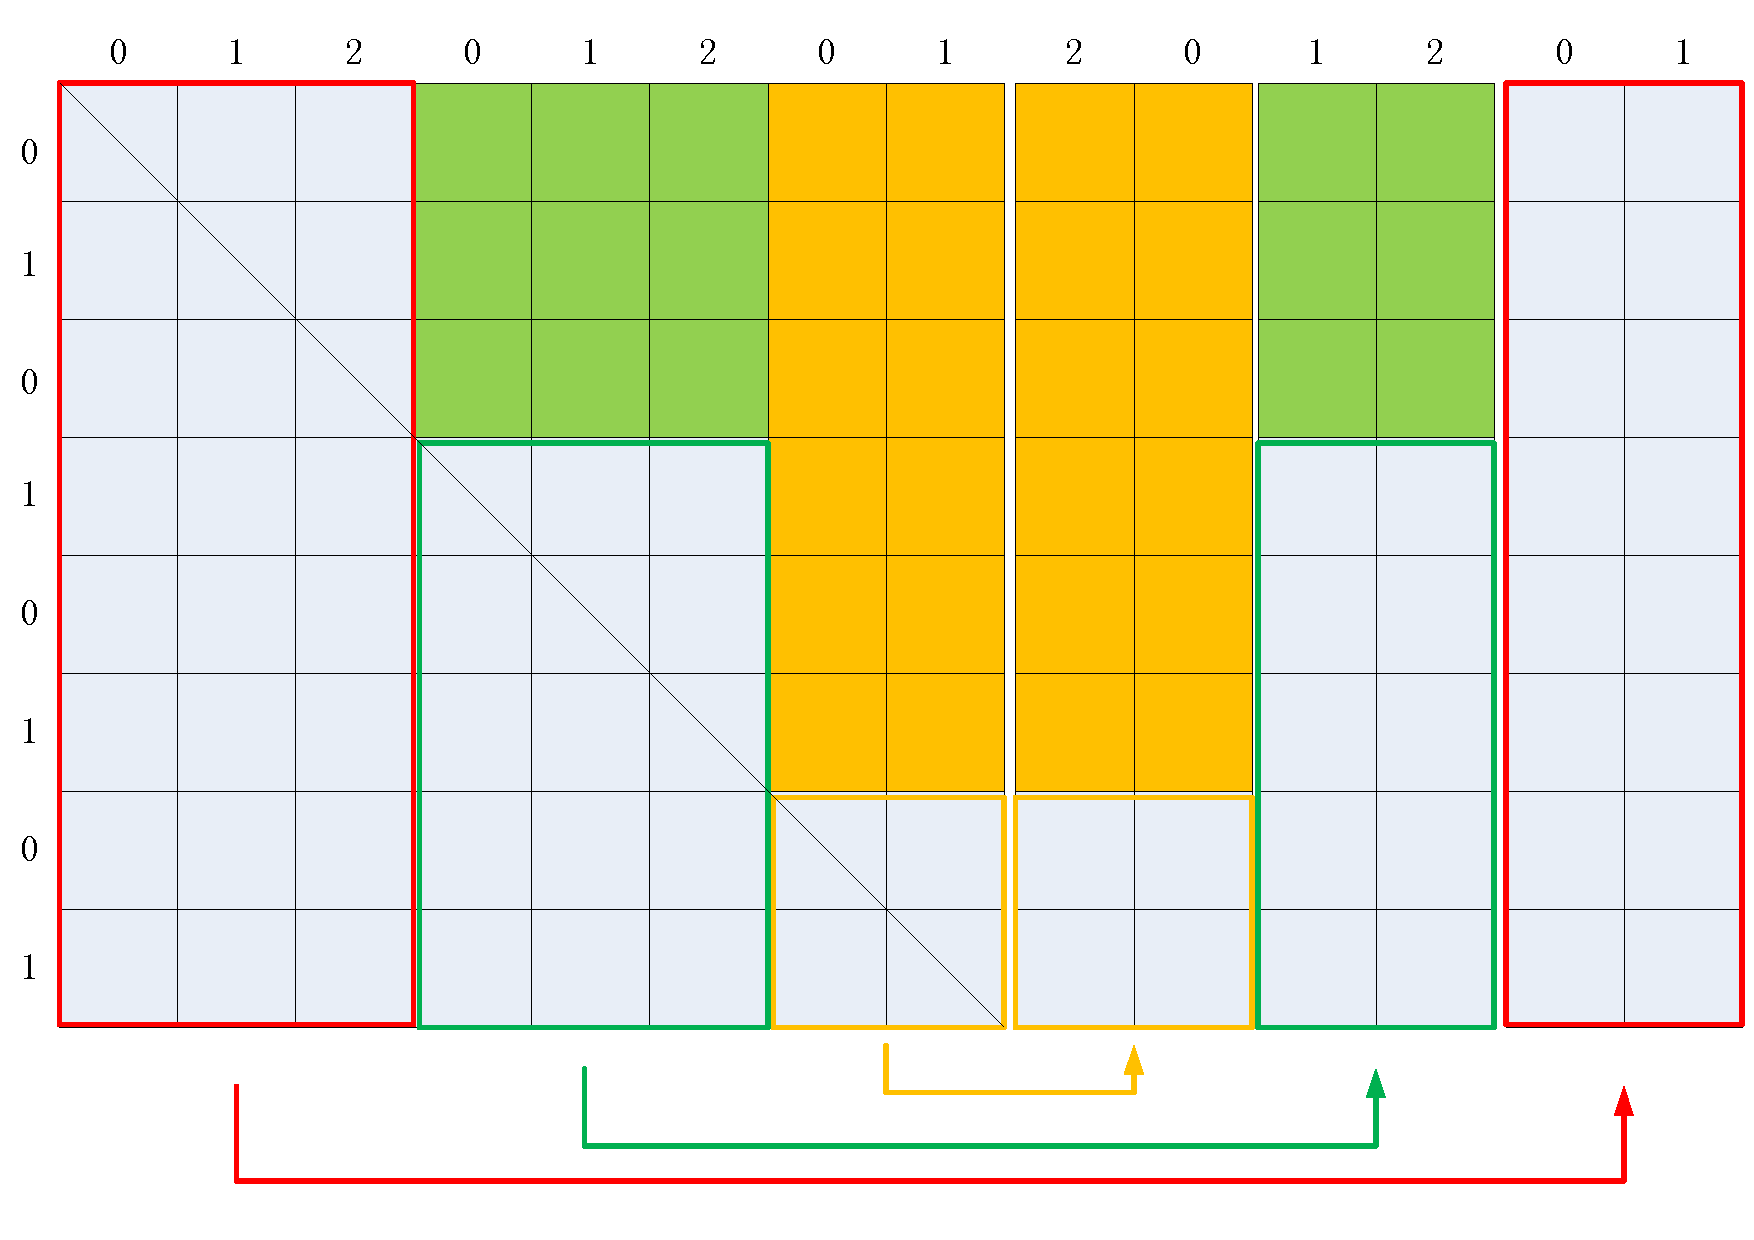
\includegraphics[width=.8\linewidth]{figures/hybrid-chpt-2x3}
    \caption{Pattern to store checksums to prevent data loss in the event of multiple failures. Figure borrowed from~\cite{pengduppopp12}}.
    \label{fig:cof:checksum}
\end{figure}

When a process failure is detected, all remaining processes are alerted of the 
location of the failure by FT-MPI, which creates a replacement process in the 
same coordinates in the $P \times Q$ block-cyclic distribution as the failed 
process. To restore any missing checksums, the value is simply copied from a 
duplicate. To restore the missing data blocks within the right factor of the 
matrix, a reduction operation calculates the value of the missing data by 
subtracting the remaining data values from the checksum. The value of the left 
factor is also stored in a checksum at the bottom of the matrix. Those values 
are either recovered from the checksum similarly to the right factor, or the 
most recent panel is recomputed.

While this algorithm was successful using FT-MPI, as previously stated, FT-MPI 
does not remain a viable candidate for MPI fault tolerance in the future. The 
algorithm was ported to a more compliant version of MPI, Checkpoint-on-Failure, 
to demonstrate its feasibility on existing systems.

\subsection{Checkpoint-on-Failure QR}

\paragraph*{Checkpoint Procedure:} 
Compared to a regular fault tolerance tool, \cof is not a standard checkpointing 
procedure. Where system-level checkpoints save the contents of large sections of 
memory, whether the data is still useful or not, \cof applications should only 
checkpoint the most vital pieces of data that are either required for an 
application to resume, or are prohibitively expensive to recalculate at recovery 
time. This means that codes should refactor their existing checkpointing 
functions to save less data and store it in a different location (depending on 
the type of application and execution environment). For \cof-QR, the 
checkpointing function saves the local values of the matrices and the loop 
indices necessary to restart. All other data critical to the application can be 
regenerated quickly from these most important pieces.

\paragraph*{State Restoration:} 
ScaLAPACK programs have deep call stacks,
including functions from several software packages, such as
PBLAS~\cite{Choi:1995:PSP:898829}, BLACS~\cite{Dongarra:1991vn, Dongarra:1995uu}, LAPACK~\cite{Anderson:1990th} and BLAS~\cite{Choi:1996wy}.
In the previously existing FT-MPI version of the QR algorithm, regardless of
when the failure was detected, the current iteration of the algorithm needed to
be completed before processing the recovery procedure. This would ensure an
identical call stack on every process and that all processes had updated their
checksums completely. For the new \cof version of QR, failure must interrupt the
algorithm immediately, not completing the current iteration, because the MPI
library can no longer support the communication necessary to calculate the most
up to date checksums. While this has the potential to cause divergent call
stacks among the processes, because failure notification happens only in MPI and
the lower level procedures (BLAS, LAPACK, etc.) do not perform communication,
the data remains uncorrupted by failures.

To resolve the call stack issue, when restarted, every process undergoes a ``dry
run'' phase where the algorithm mimics the loop nests of the QR algorithm down
to the PBLAS level without actually applying modifications to or exchanging
data. When the algorithm reaches the original point of failure, the matrix content is
loaded from the checkpoint data and the algorithm is able to continue in the
same manner as before in the FT-MPI based code. The regular recovery procedure
is applied: the current iteration of the factorization is completed to update
all checksums and the dataset is rebuilt using the ABFT reduction.

\section{\cof Performance}\label{sect:cof:performance}

In this section, we use our Open MPI and ABFT modifications to evaluate the performance
of the \cof protocol. We use two test platforms. The first machine, ``Dancer,''
is a 16-node, development cluster in the Innovative Computing Laboratory at the 
University of Tennessee. All nodes are equipped with two 2.27GHz quad-core E5520
CPUs, with a 20GB/s Infiniband interconnect. Solid State Drive disks are used as
the checkpoint storage media. The second system is the Kraken supercomputer, a 
University of Tennessee owned machine, housed at Oak Ridge National Laboratory.
Kraken is a Cray XT5 machine, with 9,408 compute nodes. Each node has two
Istanbul 2.6 GHz six-core AMD Opteron processors, 16GB of memory, and are
connected through the SeaStar2+ interconnect. The scalable cluster file system
``Lustre'' is used to store checkpoints.

\subsection{MPI Library Overhead}\label{subsect:cof:performance:overhead}

One of the main concerns from application developers when discussing fault
tolerance is the amount of overhead introduced by the addition of fault
tolerance into any application code or intermediate libraries. Our
implementation of fault detection and notification is mostly implemented in the
non-critical ORTE runtime. Typical HPC systems feature a separated service
network (usually Ethernet based) and a performance interconnect; hence health
monitoring traffic, which happens in the OOB service network, is physically
separated from the MPI communications, removing the possibility of introducing
network jitter due to fault tolerance messages. In addition, changes to the MPI
functions are minimal: the same condition that previously triggered
unconditional aborts has now been repurposed to trigger error handlers. As
expected, no impact on MPI bandwidth or latency was measured.
The memory usage of the MPI library is slightly increased, as the incarnation
number doubles the size of the process names. However, this is negligible in
typical deployments.

\subsection{Failure Detection}\label{subsect:cof:performance:detection}

Critical to the functionality of \cof is the reliable and expedient detection of
process failures. The asynchronous failure notification described in
Section~\ref{subsect:cof:ompi:notification}, provides this failure detection. We
designed a micro-benchmark to measure failure detection time as experienced by
MPI processes. The benchmark code synchronizes with an \mpifunc{MPI\_BARRIER},
stores the reference time, injects a failure at a specific rank, and enters a
ring algorithm until the MPI error handler stores the detection time. The OOB
routing topology used by the ORTE runtime introduces a non-uniform distance to
the failed process, hence failure detection time experienced by a process may
vary with the position of the failed process in the OOB topology.

\begin{figure}[t]
    \centering 
    \subfigure[Linear OOB Routing]{
		\label{fig:cof:linear-oob}
		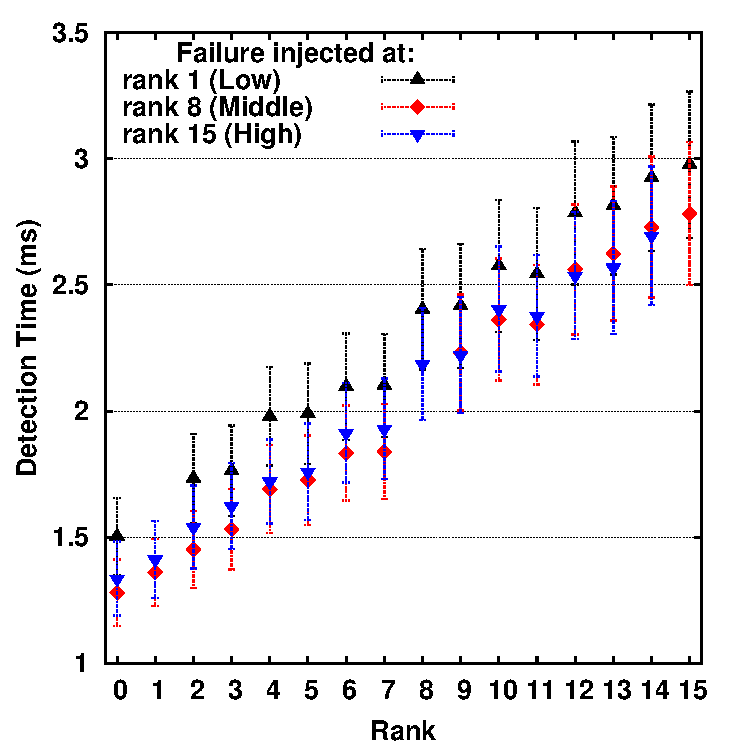
\includegraphics[width=.45\linewidth]{figures/failure-detection-linear-errbars}
	}
	\hfill
    	\subfigure[Binomial OOB Routing]{
		\label{fig:cof:binomial-oob}
    		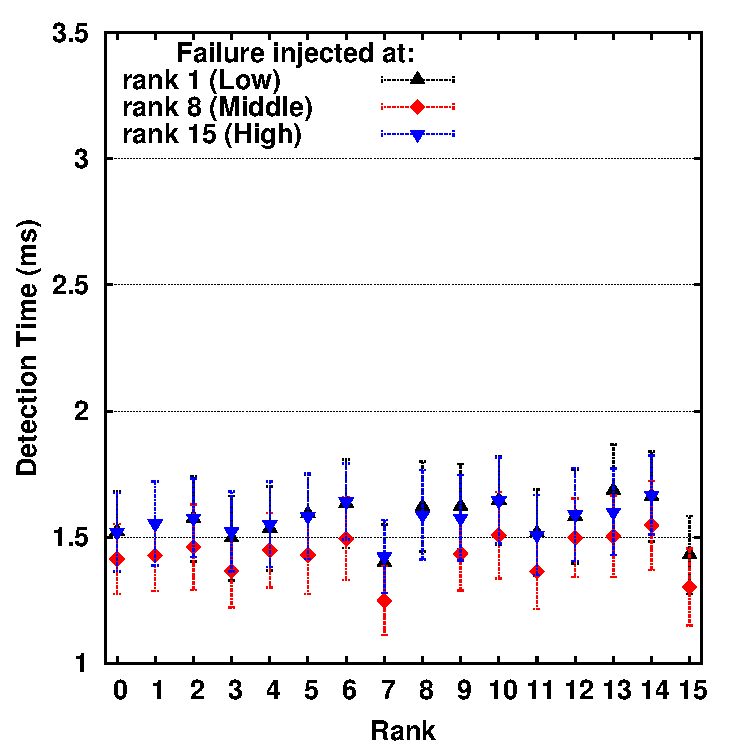
\includegraphics[width=.45\linewidth]{figures/failure-detection-binomial-errbars}
    	}
    \caption{Failure detection time, sorted by process rank, depending on the OOB 
    overlay network used for failure propagation.}
    \label{fig:cof:detection}
\end{figure}

Figures~\ref{fig:cof:linear-oob} and~\ref{fig:cof:binomial-oob} present the
failure detection times of the linear and binomial OOB topologies, respectively.
The curves ``Low, Middle, and High'' show the behavior for failures happening at
different positions in the OOB topology with ``Low'' failures being injected at 
rank 1, ``Middle'' failures occurring at rank 8, and ``High'' failures at rank 
15. On the horizontal axis is the rank of
the detecting process, and on the vertical axis is the detection time
experienced. The experiment uses 16 nodes, with one process per node, MPI over
Infiniband, OOB over Ethernet, an average of 20 runs, and the MPI barrier
latency is four orders of magnitude lower than the measured values.

In the linear topology (Figure~\ref{fig:cof:linear-oob}), every runtime process
is connected to the \emph{mpirun} process. For a higher rank, failure detection
time increases linearly because it is notified by the \emph{mpirun} process only
after the notification has been sent to all lower ranks. Obviously, this OOB 
topology is not designed to be a scalable solution. 

The binomial tree topology
(Figure~\ref{fig:cof:binomial-oob}) exhibits a similar best failure detection
time. However, this more scalable topology has a low output degree and
eliminates most contentions on outgoing messages, resulting in a more stable,
lower average detection time, regardless of the failure position. Overall,
failure detection time is on the order of milliseconds, a much smaller figure
than the typical checkpoint time.

\subsection{Checkpoint-on-Failure QR Performance}
\label{subsect:cof:performance:qr}

\begin{figure}[t]
    \centering
    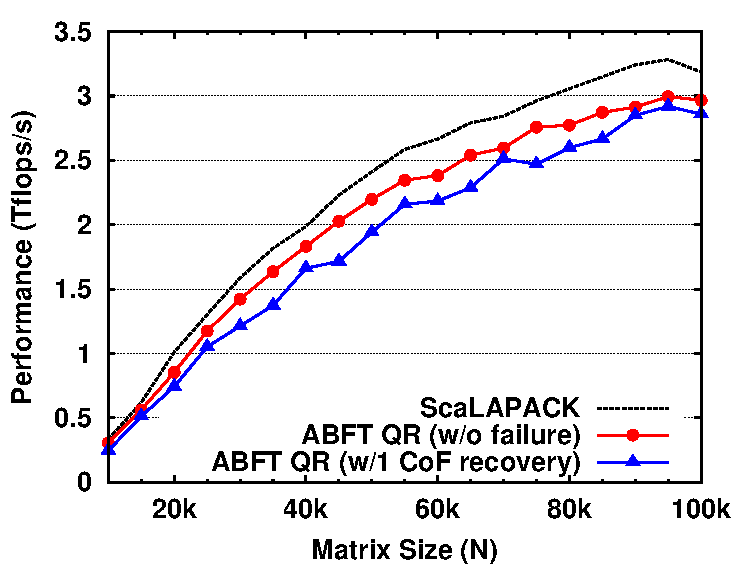
\includegraphics[width=.8\linewidth]{figures/kraken-new-data}
    \caption{ABFT QR and one \cof recovery on Kraken (Lustre).}%($24\times 24$ grid)
    \label{fig:cof:kraken-performance}	
\end{figure}

\paragraph*{Supercomputer Performance:} Figure~\ref{fig:cof:kraken-performance}
presents the performance on the Kraken supercomputer. The process grid is $24
\times 24$ and the block size is 100. The \abft QR (w/o failure) curve presents 
the performance of the \abft QR implementation, using \cof techniques, in a 
fault-free execution; it is noteworthy that when there are no failures, the 
performance is exactly identical to the performance of the unmodified \abft QR 
implementation with FT-MPI. The \abft QR (w/1 \cof recover) curve presents the 
performance when a failure is injected after the first step of the PDLARFB 
kernel. The performance of the non-fault tolerant ScaLAPACK QR is also presented 
for reference.

Without failures, the performance overhead compared to the regular ScaLAPACK is
caused by the extra computation to maintain the checksums inherent to the \abft
algorithm~\cite{pengduppopp12}; this extra computation is unchanged between
ABFT-QR without failures and ABFT-QR with a failure. Only on runs when a failure happened do the \cof protocols
undergo the supplementary overhead of storing and reloading checkpoints.
However, the performance of the \cof-QR remains very close to the no-failure
case. For instance, at matrix size N=100,000, \cof-QR still achieves 2.86
Tflop/s after recovering from a failure, which is 90\% of the performance of the
non-fault tolerant ScaLAPACK QR. This demonstrates that the \cof protocol
enables efficient, practical recovery schemes on supercomputers.

\begin{figure}[t]
	\centering
    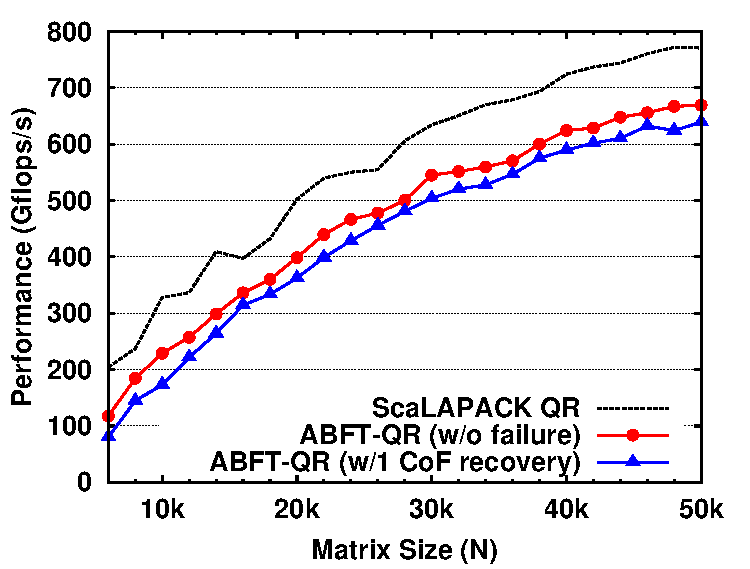
\includegraphics[width=.8\linewidth]{figures/dancer-performance-data}
    \caption{ABFT QR and one \cof recovery on Dancer (local SSD).}    	\label{fig:cof:dancer-performance}
\end{figure}

\begin{figure}[t]
	\centering
    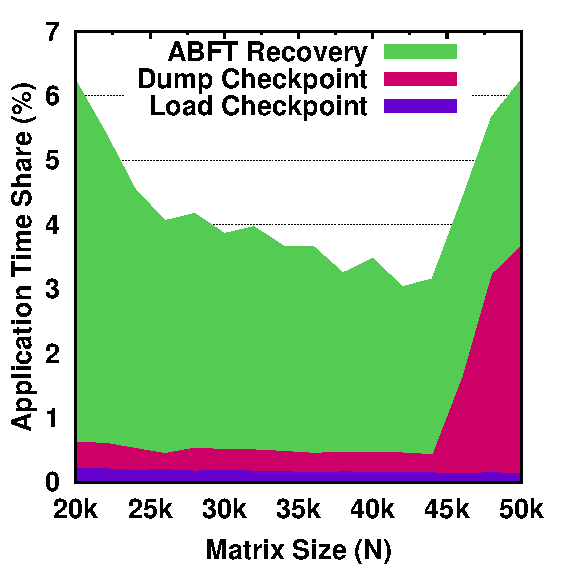
\includegraphics[width=.8\linewidth]{figures/dancer-1-error-timing-process-new-data}
    \caption{Time breakdown of one \cof recovery on Dancer (local SSD).}
    \label{fig:cof:dancer-timing}
\end{figure}

\paragraph*{Impact of Local Checkpoint Storage:}
Figure~\ref{fig:cof:dancer-performance} presents the performance of the \cof-QR
implementation on the Dancer cluster with an $8 \times 16$ process grid. Although
a smaller test platform, the Dancer cluster features local storage on nodes and
a variety of performance analysis tools unavailable on Kraken. As expected, the 
\abft method has a higher relative cost on this
smaller machine, but compared to the Kraken platform, the relative cost of \cof
failure recovery is smaller on Dancer. Like all algorithms involving 
checkpointing, the \cof protocol incurs disk access overheads to
store and load checkpoints when a failure hits, hence the recovery overhead
depends on I/O performance. By breaking down the relative cost of each recovery
step in \cof, Figure~\ref{fig:cof:dancer-timing} shows that checkpoint saving
and loading only take a small percentage of the total run-time, thanks to the
availability of solid state disks on every node. Since checkpoint reloading
immediately follows checkpointing, the OS cache satisfies most disk access,
resulting in high I/O performance. For matrices larger than N=44,000, the memory
usage on each node is high and decreases the available space for disk cache,
explaining the decline in I/O performance and the higher cost of checkpoint
management. Overall, the presence of fast local storage can be leveraged by the
\cof protocol to speedup recovery (unlike periodic checkpointing, which depends
on remote storage by construction). Nonetheless, as demonstrated by the
efficiency on Kraken, while this is a valuable optimization, it is not a
mandatory requirement for satisfactory performance.

\section{Evaluation of \cof}\label{sect:cof:evaluation}

Clearly, \cof does not meet all of the goals from Chapter~\ref{chap:goals}. It
provides relatively little \textbf{flexibility} due to the fact that it can only
write a checkpoint after discovering a failure. It does not provide a platform
to build other fault tolerance solutions. It provides sufficient \textbf{resilience} 
as it does allow the application to repair its execution by
reloading the data it writes after a failure. This allows the application to
continue executing even after a failure. Its greatest 
strength lies in its \textbf{productivity}. \cof is supported by existing MPI 
libraries and uses the familiar checkpointing paradigm as its basis. To that 
end, it is easily adopted by current applications as a possible solution for 
fault tolerance. A number of linear algebra algorithms can quickly adopt the tools in 
\cof with relatively little modification: one-sided factorizations, iterative conjugate 
gradient methods, and two-sided factorizations. The only changes necessary are to 
minimize the checkpoint size and to write a function to algorithmically repair the 
missing data. 
